\PassOptionsToPackage{dvipsnames}{xcolor}
\PassOptionsToPackage{oneside}{geometry}
\documentclass[twocolumn, twocolappendix, oneside]{aastex631}
\received{\today}
\shorttitle{Imprints of mass transfer on asteroseismic signals}
\graphicspath{{figures/}}

\usepackage{lipsum}
\usepackage{physics}
\usepackage{multirow}
\usepackage{xspace}
\usepackage{natbib}
\usepackage{fontawesome5}
\usepackage{wrapfig}
\usepackage[figuresright]{rotating}

% remove indents in footnotes
\usepackage[hang,flushmargin]{footmisc} 

\usepackage{styles/todo_notes}

% \newcommand{\todo}[1]{{\color{red}{[TODO: #1}]}}
% \newcommand{\needcite}{{\color{magenta}{(needs citation)}}}
\newcommand{\placeholder}[1]{{\color{gray} \lipsum[#1]}}
\newcommand{\paraOutlineHdr}[1]{{\color{gray}[\textit{#1}]}}

% custom function for adding units
\makeatletter
\newcommand{\unit}[1]{%
    \,\mathrm{#1}\checknextarg}
\newcommand{\checknextarg}{\@ifnextchar\bgroup{\gobblenextarg}{}}
\newcommand{\gobblenextarg}[1]{\,\mathrm{#1}\@ifnextchar\bgroup{\gobblenextarg}{}}
\makeatother

% shorthands
\renewcommand{\bv}{Brunt–Väisälä\xspace}
\newcommand{\bvf}{Brunt–Väisälä frequency\xspace}
\newcommand{\hrd}{Hertzsprung-Russell diagram\xspace}
\newcommand{\gmode}{$g$-mode\xspace}
\newcommand{\gmodes}{$g$-modes\xspace}
\newcommand{\mesa}{\texttt{MESA}\xspace}

\newif\ifstartedinmathmode
\newcommand{\msun}{%
  \relax\ifmmode\startedinmathmodetrue\else\startedinmathmodefalse\fi
  {\ifstartedinmathmode\unit{M_{\odot}}\else$\unit{M_{\odot}}$\fi}\xspace%
}

\newif\ifstartedinmathmode
\newcommand{\rsun}{%
  \relax\ifmmode\startedinmathmodetrue\else\startedinmathmodefalse\fi
  {\ifstartedinmathmode\unit{R_{\odot}}\else$\unit{R_{\odot}}$\fi}\xspace%
}

\definecolor{dark}{rgb}{0.2,0.2,0.2}
\newcommand{\darkmode}{
    \pagecolor{dark}
    \color{white}
    \hypersetup{linkcolor=yellow,urlcolor=yellow,
                anchorcolor=yellow,citecolor=yellow}
}

\begin{document}

% \darkmode{}

\title{The Asteroseismic Imprints of Mass Transfer}

% affiliations
\newcommand{\UW}{\affiliation{Department of Astronomy, University of Washington, Seattle, WA, 98195}}
\newcommand{\mpa}{\affiliation{Max-Planck-Institut für Astrophysik, Karl-Schwarzschild-Straße 1, 85741 Garching, Germany}}
\newcommand{\yale}{\affiliation{Department of Astronomy, Yale University, CT, 06511, USA}}
\newcommand{\cca}{\affiliation{Center for Computational Astrophysics, Flatiron Institute, 162 Fifth Ave, New York, NY, 10010, USA}}
\newcommand{\radbound}{\affiliation{Department of Astrophysics, IMAPP, Radboud University Nijmegen, PO Box 9010, 6500 GL Nijmegen, The Netherlands}}
\newcommand{\leuven}{\affiliation{Institute of Astronomy, KU Leuven, Celestijnenlaan 200D, 3001 Leuven, Belgium}}

\author[0000-0001-6147-5761]{Tom Wagg}
\UW{}
\mpa{}

\author[0000-0002-3054-4135]{Cole Johnston}
\radbound{}
\leuven{}

\author[0000-0003-4456-4863]{Earl P. Bellinger}
\mpa{}
\yale{}

\author[0000-0002-6718-9472]{Mathieu Renzo}
\cca{}

\author[0000-0001-9336-2825]{Selma E. de Mink}
\mpa{}

\correspondingauthor{Tom Wagg}
\email{tomjwagg@gmail.com}

\begin{abstract}
    We present new simulations investigating the impact of mass transfer on the asteroseismic signals of slowly pulsating B stars. We use \mesa to simulate the evolution of a binary star system and \texttt{gyre} to compute the asteroseismic properties of the accretor star. We show that, compared to a single star of the same final mass, a star that has undergone accretion has a significantly different internal structure, evident in both the hydrogen abundance profile and \bvf profile. These differences result in significant changes in the observed period spacing patterns, implying that one may use this as a diagnostic to test whether a star's core has been rejuvenated as a result of accretion. We show that one may draw misleading conclusions of stellar properties when only assuming single star evolution in fitting procedures. Our proof of principle analysis demonstrates the need to further investigate the impact of binary interactions on stellar asteroseismic signals for a wide range of parameters, such as initial mass, amount of mass transferred and the age of the accretor star at the onset of mass transfer.
\end{abstract}

\keywords{Asteroseismology, Binary stars, Accretion, Interacting binary stars, Multiple star evolution, Stellar evolution, Roche lobe overflow}

{\hypersetup{linkcolor=black}\listoftodos}

\clearpage

\section{Introduction} \label{sec:intro}

% Cole says: Just looking at your introduction, and I think that I would flip the order of information here -- put right up front that all (massive) stars are in binaries and that we expect a large portion of them to undergo at least one phase of mass transfer. This leaves large uncertainties in evolutionary calculations and predictions, for instance relating to the production of close double compact object binaries and gravtiational wave sources. Therefore, it is very important that we understand how mass transfer impacts the structure and evolution of stars.
% There's a lot of work done on understanding the diversity of mass-losers, but there are still many uncertainties for the mass gainers. One of the more important uncertainties is whether or not a star will be rejuvenated. We don't have a proper observational diagnostic for determining whether the core of a star has been rejuvenated. Enter asteroseismology!

The majority of massive stars are born in binaries and multiple systems \citep[e.g.][]{Mason+2009, Almeida+2017, Moe+2017}, a large subset of which will exchange mass \citep[e.g][]{Sana+2012}. However, mass transfer, both the process itself and the impact it has on the component stars, is still highly uncertain. This means that there are large uncertainties in evolutionary calculations and predictions, such as the rate of formation of close double compact objects and gravitational wave sources \citep[e.g.][]{Broekgaarden+2022}.

There are still many uncertainties in the effect that mass transfer has on mass-gainers, despite the many investigations into understanding the diversity of mass-losers.\cole{Could you point me to some of these or a starting paper I can use to find the rest?}Among these uncertainties a key question is whether a mass-gainer will be rejuventated, where convective cores in accretors grow to account for the additional mass \citep[e.g.][]{Neo+1977}, and if so, to what extent. To date, there is no strong observational diagnostic for determining whether the core of a star has been rejuvenated.

Asteroseismology probes the internal structure of stars and so may hold the key to constraining rejuvenation. It is well established that asteroseismology can be used to estimate precise stellar masses, radii and ages based on stellar oscillation modes \citep{Aerts+2010}. In particular, main sequence gravity ($g$) mode pulsators can be observed deep into their radiative envelopes using high-order \gmode oscillations. These pulsators include Slowly Pulsating B (SPB) stars, driven by the $\kappa$-mechanism \citep{Waelkens+1985, Waelkens+1991, Cox+1992, Pamyatnykh+1999}.
% These pulsators include $\gamma$ Doradus stars driven by the modulation of the radiative flux by convection at the base of a deep envelope convection zone \citep{Guzik+2000}, and Slowly Pulsating B (SPB) stars and $\beta$ Ceph stars driven by the $\kappa$-mechanism \citep{Waelkens+1985, Waelkens+1991, Kiriakidis+1992, Moskalik+1992, Cox+1992}.
\gmode pulsators have been used to provide insights into many aspects of stellar evolution, such as the mass of stellar cores \citep{Johnston+2021, Pedersen+2022} internal mixing processes, and angular momentum transport \citep{Aerts+2019}. Recently, \gmode asteroseismology has been used to probe the chemical and temperature gradients outisde of the cores of massive stars \citep{Michielsen+2021, Pedersen+2018}.

These insights into stellar properties are possible due to the intricate dependence of period spectrum of \gmode pulsations on the size of the convective core and the chemical composition gradient outside of the core \citep[e.g.][]{Miglio+2008}. Based on these measured properties, one can infer precise estimates of stellar masses and radii, as well as stellar ages and internal structure properties with additional assumptions of stellar evolution.

Current works only consider single star evolution when inferring stellar properties. However, mass transfer can profoundly influence the structure and composition gradients of accreting stars even after thermal re-adjustment, as indicated by numerous studies using 1D stellar evolution codes \citep{Renzo+2021, Miszuda+2021}. These changes in structure are usually a result of rejuvenation.

As the frequencies of self-excited stellar pulsations are finely tuned by the internal structure of stars, asteroseismology holds the potential to identify the signature of previous mass transfer in various classes of pulsating stars. Furthermore, assuming single star evolution for a star that has undergone accretion may result in misleading inferences of its stellar properties from asteroseismology.

In this paper we assess the impact that mass transfer leaves on the asteroseismic signal of pulsating stars that have recently gained mass through binary interaction. In particular we focus on SPB stars as they are numerous, easily observationally identifiable and have a relatively high binary fraction. We use the 1D stellar evolution code \mesa to demonstrate the difference in evolution between an accreting star and an equivalent single star. Using the \texttt{GYRE} stellar oscillation code we show how these differences in evolution influence the period spacing pattern of an accreting star and highlight how this could affect the inferred properties of the star if single stellar evolution was assumed.

% \section{Old Introduction} \label{sec:intro}

% Motivation: Asteroseismology is important
% \paraOutlineHdr{Asteroseismology is cool and probes internal stellar structure}
% Asteroseismology is a well established method for estimating precise stellar masses, radii and ages based on stellar oscillation modes \citep{Aerts+2010}. In particular, asteroseismology is capable of probing the internal structure of observed stars.

% \paraOutlineHdr{\gmode pulsators are useful}
% In particular, main sequence gravity ($g$) mode pulsators can be observed deep into their radiative envelopes using high-order \gmode oscillations. These pulsators include $\gamma$ Doradus stars driven by the modulation of the radiative flux by convection at the base of a deep envelope convection zone \citep{Guzik+2000}, and Slowly Pulsating B (SPB) stars and $\beta$ Ceph stars driven by the $\kappa$-mechanism \citep{Waelkens+1985, Waelkens+1991, Kiriakidis+1992, Moskalik+1992, Cox+1992}. These stars can be used to provide insights into many aspects of stellar evolution such as angular momentum transport efficiency \citep[e.g.][]{Aerts+2019}.

% \paraOutlineHdr{Asteroseismology probes convective core size and composition gradients}
% These insights into stellar properties are possible due to the intricate dependence of period spectrum of \gmode pulsations on the size of the convective core and the chemical composition gradient outside of the core \citep[e.g.][]{Miglio+2008}.
% %This dependence comes from the fact that \gmode pulsations obey a dispersion relation involving the buoyancy (\bv) frequency.
% Based on these measured properties, one can infer precise estimates of stellar masses and radii, as well as stellar ages with additional assumptions of stellar evolution.

% The potential problem: mass transfer may affect inferred properties
% \paraOutlineHdr{Current work uses SSE, but accretion changes things!}
% Current works only consider single star evolution when inferring stellar properties. However, mass transfer can profoundly influence the structure and composition gradients of accreting stars even after thermal re-adjustment, as indicated by numerous studies using 1D stellar evolution codes \citep{Renzo+2021, Miszuda+2021}. These changes in structure are usually a result of ``rejuvenation'', where convective cores in accretors grow to account for the additional mass \citep[e.g.][]{Neo+1977}.

% \paraOutlineHdr{Lots of pulsators undergo accretion, this has implications} 
% Given the typical masses of \gmode pulsators, we expect that a significant fraction of them are born in multiple systems \citep[e.g.][]{Mason+2009, Almeida+2017, Moe+2017}, a large subset of which will exchange mass \citep[e.g][]{Sana+2012}. As the frequencies of self-excited stellar pulsations are finely tuned by the internal structure of stars, asteroseismology holds the potential to identify the signature of previous mass transfer in various classes of pulsating stars. Furthermore, assuming single star evolution for a star that has undergone accretion may result in misleading inferences of its stellar properties from asteroseismology.

% Our contribution: we investigate the effect of mass transfer
% \paraOutlineHdr{We test the impact of mass transfer}
% In this paper we assess the impact that mass transfer leaves on the asteroseismic signal of pulsating stars that have recently gained mass through binary interaction. In particular we focus on SPB stars as they are numerous, easily observationally identifiable and have a relatively high binary fraction. We use the 1D stellar evolution code \mesa to demonstrate the difference in evolution between an accreting star and an equivalent single star. Using the \texttt{GYRE} stellar oscillation code we show how these differences in evolution influence the period spacing pattern of an accreting star and highlight how this could affect the inferred properties of the star if single stellar evolution was assumed.

% \tom{Follow Cole's advice in flipping the order of information}

\section{Binary Stellar Evolution} \label{sec:methods}

In this Section we outline the setup of our \mesa binary models and describe the evolution of the system, both across the \hrd and in terms its internal structure.

\subsection{Model setup}

We use Modules for Experiments in Stellar Astrophysics \citep[\mesa,][]{Paxton2011, Paxton2013, Paxton2015, Paxton2018, Paxton2019, Jermyn2023} version r23.05.01 \citep{mesa_zenodo} to simulate non-rotating models for a binary system, as well as a grid of single stars against which to compare. Our full inlists are available on GitHub\footnote{\url{https://github.com/TomWagg/mass-gainer-seismology}} and our model outputs are available on Zenodo\footnote{\url{https://zenodo.org/record/}}.\tom{add Zenodo links when done}

In particular, the most pertinent settings that we change from the defaults for this work are as follows: We adopt the \citet{Ledoux+1947} criterion to account for the presence of a chemical gradient when determining the stability of convection. We include semiconvection following \citet{Langer+1983} with a scaled efficiency of $\alpha_{\rm thm}=0.1$. For accretors we include thermohaline mixing once they finish accretion following \citet{Kippenhahn+1980} with an efficiency of $\alpha_{\rm SC} = 1$. We use exponential core overshooting from \cite{Herwig+2000}, setting $(f, f_0) = (0.01, 0.005)$ \citep{Claret+2017}. We set a minimum diffusive mixing coefficient of $20~\unit{cm^{2} ~s^{-1}}$; this smooths out any numerical discontinuities in the composition gradients and accounts for a lack of rotational mixing in our models. We motivate our choice of $20~\unit{cm^{2} ~s^{-1}}$ and highlight the effect of changing the mixing coefficient on our results in Appendix~\ref{app:min_D_mix}. We follow the \citet{Kolb+1990} prescription to the mass transfer rate with an implicit scheme. We do not account for any rotation in our models. Although we expect that a typical pulsator will likely have some level of rotation, we restrict our proof of principle analysis to less complex non-rotating models. We discuss this choice further in Section~\ref{sec:caveats}.

Our binary model has a donor with an initial mass of 4\msun and an accretor with an initial mass of 3\msun, following the typical mass range of SPB stars \citep{Waelkens+1985, Waelkens+1991, Kurtz+2022}, with an initial period of 5 days and metallicity $Z = 0.02$. We evolve this system up to Roche Lobe overflow and proceed with mass transfer until the secondary accretes 0.5\msun. At this point we end mass transfer, detach the binary and reduce the donor to a point mass, since we are no longer interested in the properties of the donor and thus only track the evolution of the accretor from this point onwards. Although our choice of $0.5\msun$ is somewhat arbitrary, this amount could be obtained through different choices of mass transfer efficiencies and the spin-up of the accretor would likely hinder accretion in a similar manner. By constructing our model in this way we are able to account for a realistic, variable accretion rate. \selma{Help justify the binary model setup.} We then evolve the rejuvenated accretor until central hydrogen depletion. Additionally, for comparison, we evolve a grid of single stars with masses from 3-6\msun until the end of helium core burning.

\subsection{\hrd evolution}

\begin{figure}[htb]
    \centering
    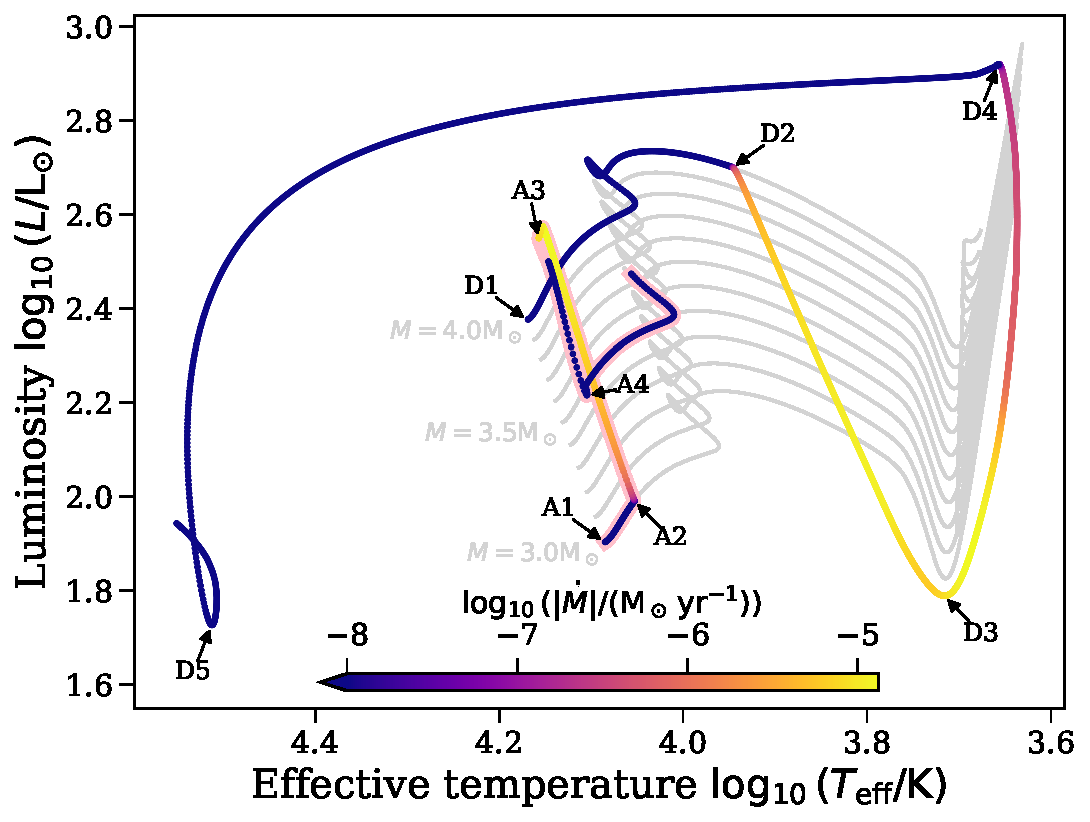
\includegraphics[width=\columnwidth]{figures/HRD_binary_full_labelled.pdf}
    \caption{\hrd showing the evolution of the binary. Tracks are shown for both the donor and accretor, coloured by the absolute mass transfer rate. We highlight the accretor track with a pink outline. Single star tracks added as background grey curves, with masses from $3$ to $4 \unit{M_\odot}$ in $0.1 \unit{M_\odot}$ intervals. Important points in the evolution are annotated with arrows and described in the text.\mathieu{Mathieu and Selma disagree on HRD}
    \selma{Mathieu and Selma disagree on HRD}}
    \label{fig:hrd}
\end{figure}

In Figure~\ref{fig:hrd} we show the evolution across the \hrd of both the donor and accretor of our binary model, with a subset of our single stellar models in the background.

The evolution of the donor (starting at D1) initially follows the 4\msun single star track, expanding across the main sequence, turning-off and moving across the Hertzsprung gap. Midway through the expansion on the Hertzsprung gap, at point D2, the donor overflows its Roche Lobe and diverges from the single star track, decreasing in luminosity as it transfers mass. As the mass transfer proceeds the orbit of the binary shrinks, increasing the mass transfer rate until the point of closest approach at D3. With the reversal of the mass ratio, mass transfer then causes the orbit the widen, decreasing the mass transfer rate and allowing the donor to increase in luminosity once more. Once the orbit widens to such an extent that Roche lobe overflow ceases (at point D4), the donor relaxes on a thermal timescale, before proceeding with helium core burning from point D5 onwards.

The evolution of the accretor (highlighted in pink) follows the 3\msun single star track initially (starting from point A1), but early into its main sequence evolution the donor initiates mass transfer (at point A2) and the accretor increases in luminosity to compensate. Once mass transfer ceases at point A3, the accretor returns to thermal equilibrium at point A4 and proceeds with its main sequence evolution along the 3.5\msun single star track.

\subsection{Rejuvenation and chemical gradients}\label{sec:xh_profiles}

\begin{figure}[tb]
    \centering
    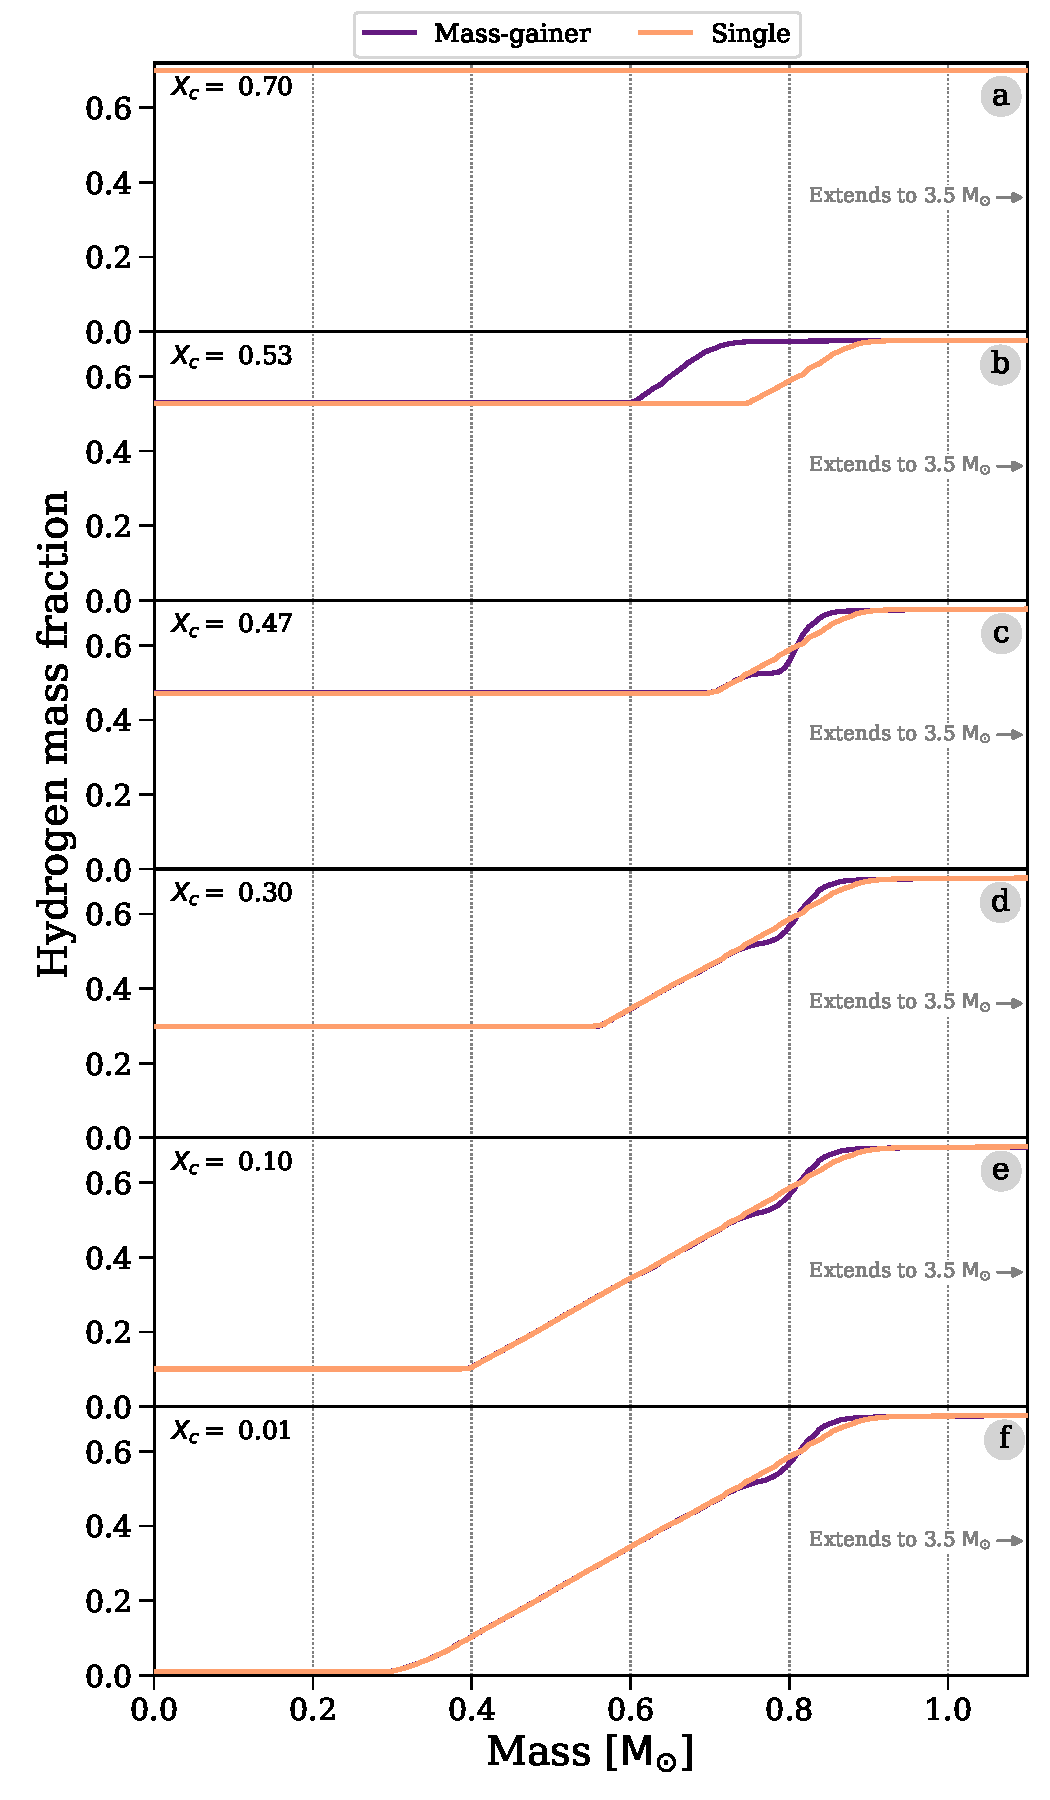
\includegraphics[width=\columnwidth]{figures/XH_profile_all.pdf}
    \caption{Comparison of the hydrogen abundance profiles between (i) an initially 3\msun star that accretes mass from a companion and (ii) a single star with the same final mass of 3.5\msun. Each panel compares the stars at the same central hydrogen abundance, which is annotated in each panel.}
    \label{fig:XH_profiles}
\end{figure}

Although the accretor appears to simply follow a more massive single star track in the \hrd, its \textit{internal} structure has been altered to support the incoming mass, leading to a rejuvenated core (). This is evident in the hydrogen abundance profile of the star, which we plot in Figure~\ref{fig:XH_profiles}. In each panel we compare the accretor of our binary model with a 3.5\msun single star, thus the stars have the same final mass. We highlight that in this figure mass transfer occurs between panels b and c and discuss the difference below.

First, we consider the evolution of the abundance profile for the single star. As the star evolves, it burns hydrogen in its core, decreasing the central hydrogen abundance. At the same time, the reduced hydrogen abundance decreases the opacity of the edge of the core, allowing radiation to travel more freely, leading to a recession of the convective core \citep{Mitalas+1972,Crowe+1982,Miglio+2008,SilvaAguirre+2011}. As the core recedes it has a decreasing hydrogen abundance, and therefore it imprints a composition gradient in its wake in the abundance profile. We see these trends in Figure~\ref{fig:XH_profiles} as the single star (shown in orange) evolves, with the central abundance decreasing and the imprinted chemical composition gradient extending over time (in the region with diagonal lines).

For the mass-gainer the evolution initially proceeds in a similar manner. In panel b, the shape is similar to that of the single star, though with a smaller convective core due to the star's initially lower mass. Between panels b and c, mass transfer occurs. As mass transfer proceeds the accretor increases in luminosity to compensate for the additional mass. This leads to an increase in the convective core size, which one can see as the profiles move outwards in mass coordinates in Figure~\ref{fig:X_H_zoom_MT}. At the same time this core expansion leads to a rejuvenation of the accretor as more hydrogen is mixed into the core, increasing the central abundance \citep{Neo+1977}. The expansion of the core into the region through which it previously receded sharpens the composition gradient, resulting in the `kink' in the abundance profile relative to the single star for the remaining panels of Figure~\ref{fig:XH_profiles}. The origin of this feature is shown in Figure~\ref{fig:X_H_zoom_MT}, where we see the hydrogen abundance increase and extend outwards as the core rejuvenates, thus washing away the previous gradient. Returning to Figure~\ref{fig:XH_profiles}, the evolution of the abundance profile after mass transfer proceeds similarly to the single star, with subsequent recession of the core and a resulting composition gradient. Critically however, the feature arising from mass transfer remains throughout the main sequence (albeit marginally smoothed by internal mixing).

\begin{figure}[tb]
    \centering
    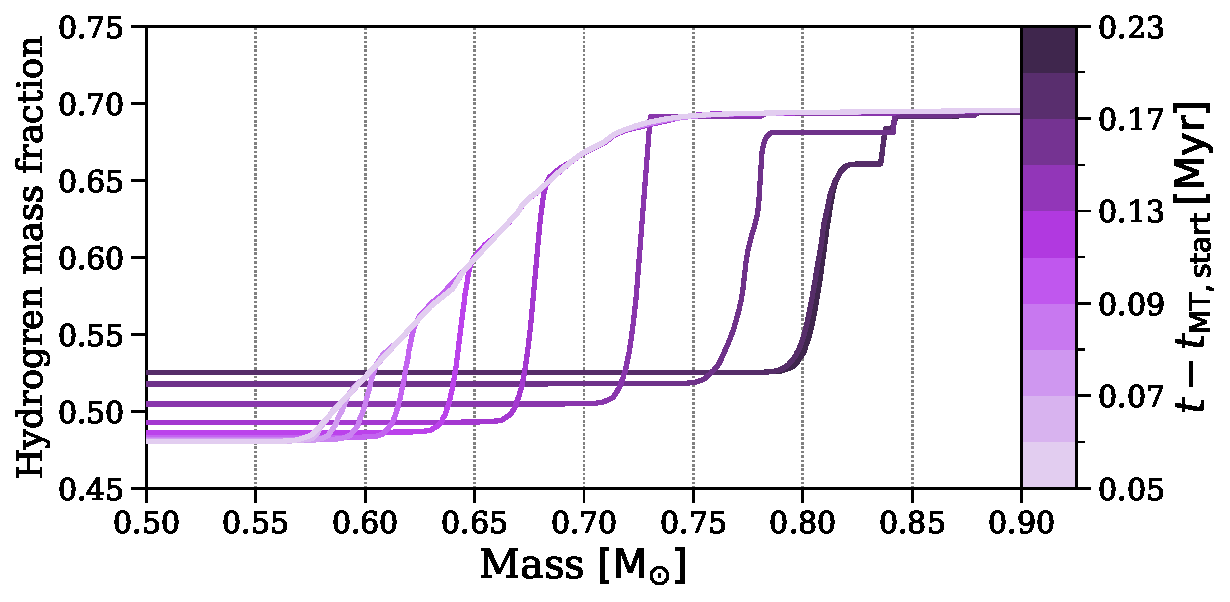
\includegraphics[width=\columnwidth]{figures/XH_profile_zoom_MT.pdf}
    \caption{Hydrogen abundance profile of our accretor model during mass transfer. Each line is coloured by its time after the start of mass transfer. This plot shows more time-resolved evolution between panels b and c of Figure~\ref{fig:XH_profiles}.}
    \label{fig:X_H_zoom_MT}
\end{figure}

\section{Asteroseismic Signals} \label{sec:results}

In this Section we demonstrate how the differences in internal structure between the accretor and single star lead to altered asteroseismic signals. We first consider how the \bvf profile is changed, before showing how this influences the period spacing patterns.

\subsection{\bvf profile}\label{sec:bvf}

% \begin{figure}[tb]
%     \centering
%     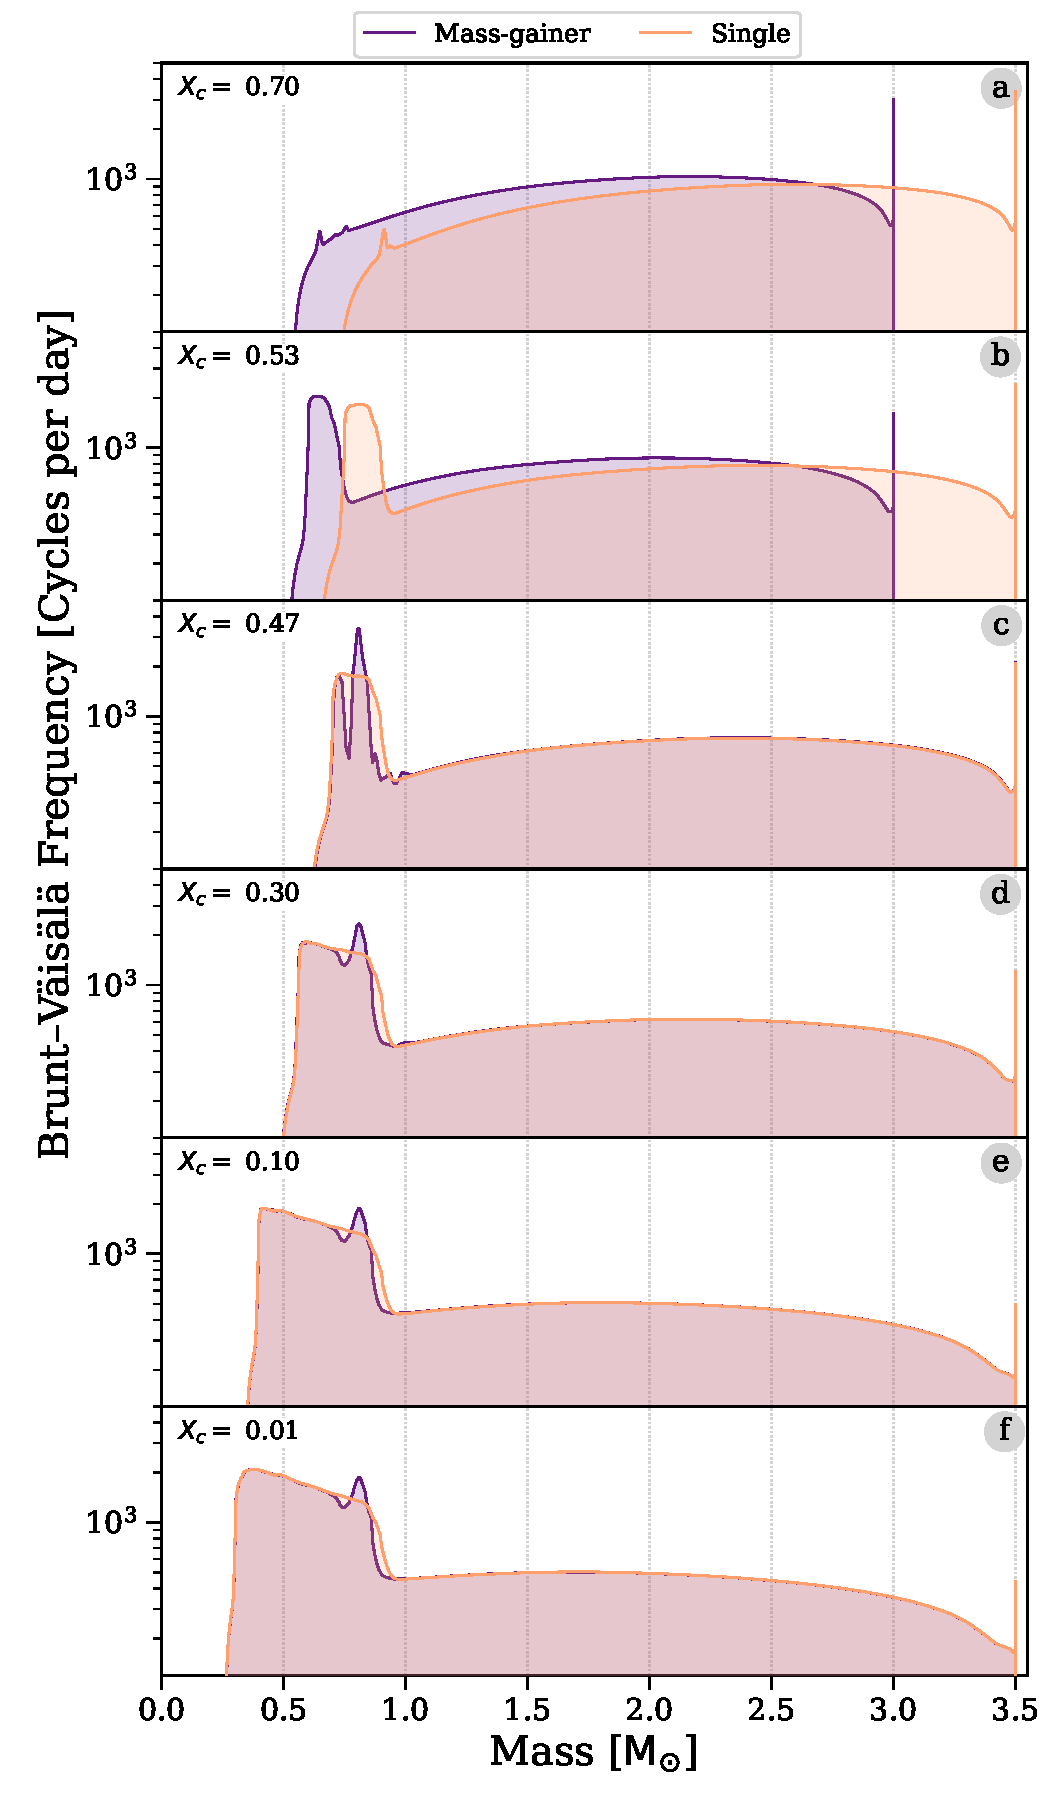
\includegraphics[width=\columnwidth]{figures/BV_profile_all.pdf}
%     \caption{As Figure~\ref{fig:XH_profiles}, but instead showing the \bvf profile.}
%     \label{fig:BV_profiles}
% \end{figure}

\begin{figure*}
    \centering
    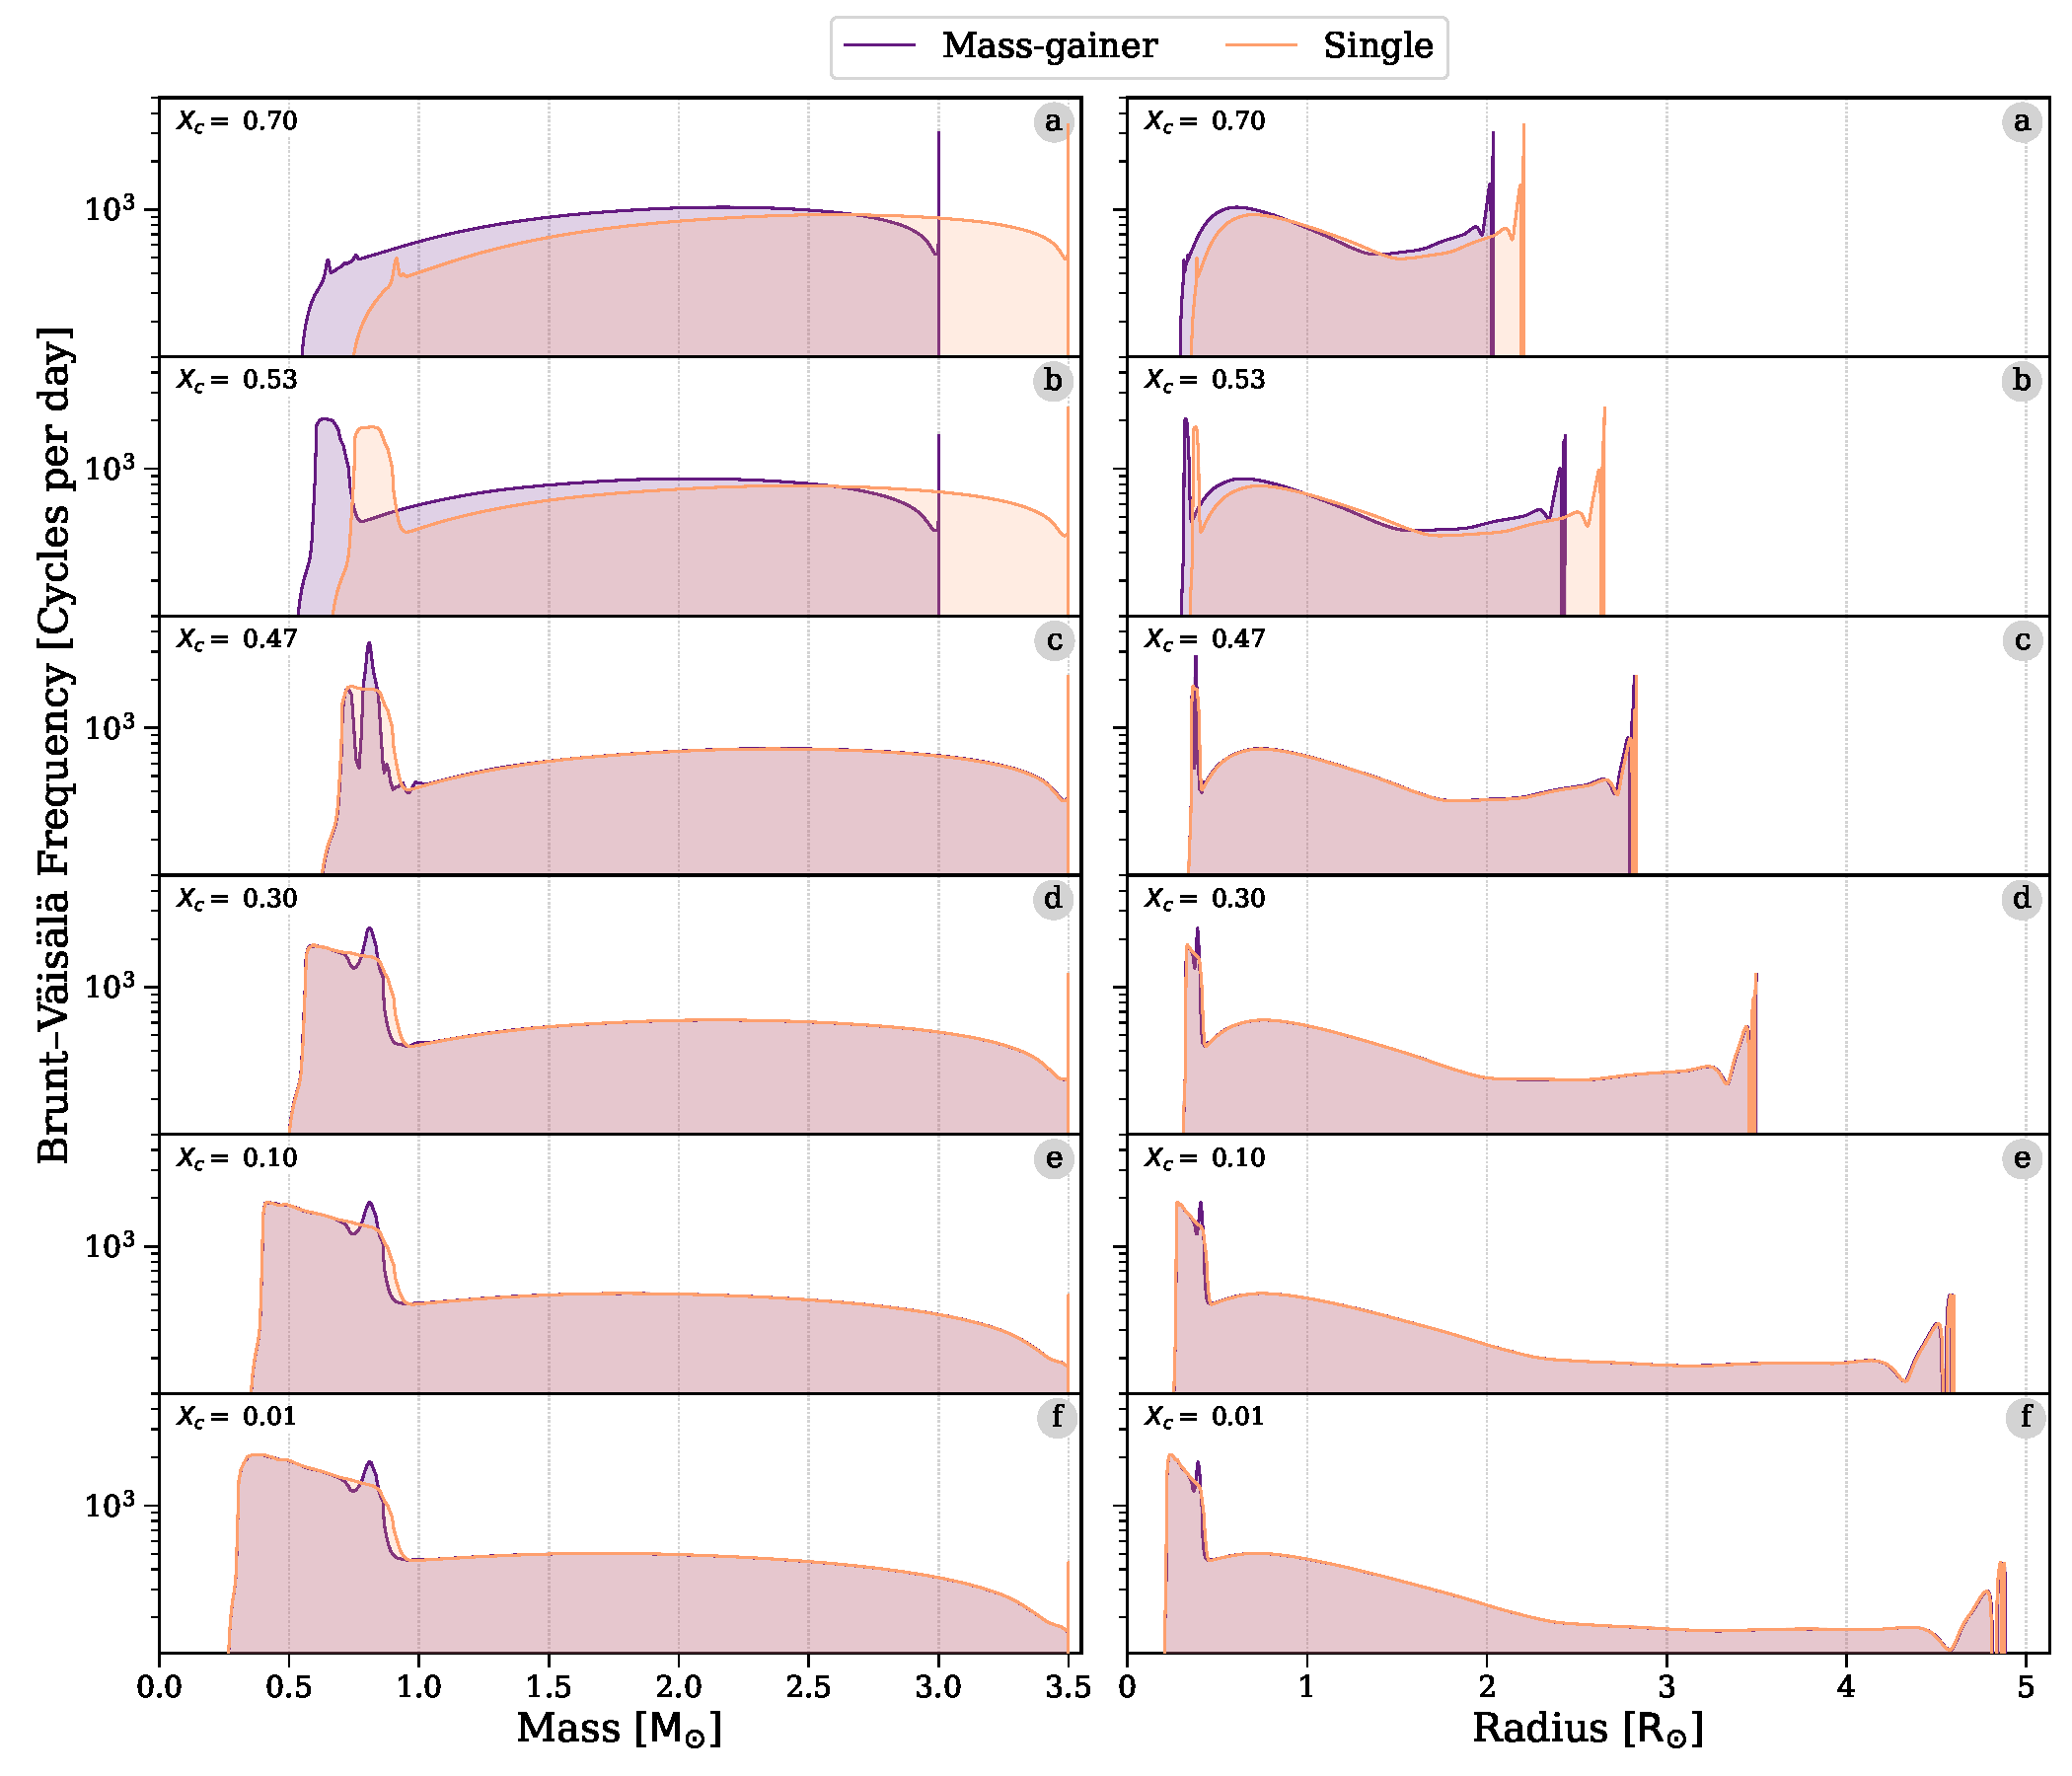
\includegraphics[width=\textwidth]{figures/BV_profile_all_combo.pdf}
    \caption{As Figure~\ref{fig:XH_profiles}, but showing the \bvf profile for the same evolutionary timesteps. \textbf{Left:} as a function of mass coordinate, \textbf{right:} as a function of radial coordinate.}
    \label{fig:BV_profiles}
\end{figure*}

The \bvf \citep{BVF-vaisala, BVF-brunt}, $N$, defines the regions in which convective instabilities can occur, such that $N^2 < 0$ indicates a convective region, and $N^2 > 0$ a radiative region in which \gmodes can propagate\footnote{The \bvf was originally derived for us in meteorology and only later applied to stellar evolution. We encourage the interested reader to read the original derivation in \citet{BVF-brunt}}. The \bvf directly determines the period distribution of \gmode oscillations and thus it is pertinent to consider the impact of mass transfer on it. For an ideal gas the frequency can be approximated as
\begin{equation}\label{eq:bvf}
    N^2 \approxeq \frac{g^2 \rho}{P} \qty(\grad_{\rm ad} - \grad + \grad_\mu),
\end{equation}
where $\rho$ is the density, $P$ is the pressure, $\grad_{\rm ad} = 2/5$ is the adiabatc temperature gradient and assumed to be a constant, $\grad$ is the temperature gradient and $\grad_\mu$ is the chemical composition gradient. We highlight that although many of the terms in this expression are similar for our accretor model and equivalent single star model, the density profile and, as noted in Section~\ref{sec:xh_profiles}, the composition gradient $\grad_\mu$ show significant differences and as such we expect similar differences in the \bvf profile.

In Figure~\ref{fig:BV_profiles} we compare, for the same central hydrogen content, the \bvf profiles for the accretor star model and single star model with the same final mass. Each panel is for the same central hydrogen content as in Figure~\ref{fig:XH_profiles} for simple comparison. We additionally show the profile as a both a function of mass coordinate and radial coordinate in the two columns.

Considering first the single star model, we see that initially the convective core ($N<0$) extends to ${\sim}$0.75\msun (or ${\sim}$0.3\rsun) and the frequency profile changes smoothly across the star. As the star evolves, the core recedes, leaving behind a chemical gradient; a peak then emerges in the \bvf profile that extends between the core and the unmixed outer regions of the star. This peak is directly due to the chemical composition gradient imprinted on the star by the receding core during the main sequence. As the star evolves, the peak extends in concert with the recession of the core, in line with the composition gradient.

For the accretor model, we see similar evolution in panels a and b (before mass transfer occurs). Immediately following mass transfer (in panel c), the convective core size aligns with the single star model and several sharp features emerge outside of the core, arising due to the kink in the composition gradient visible in panel c of Figure~\ref{fig:XH_profiles}. As the star evolves, mixing smooths these features to some extent, but importantly the star retains a double-peaked \bvf profile for the rest of its main sequence evolution.

The \bvf profile of the accretor is inaccessible through single star evolution, which would always result in a smooth, unimodal peak due to the monotonic change in central hydrogen content.

\subsection{Period spacing patterns}

All differences between the mass-gainer and equivalent single star that we have noted so far are within the internal structure, and so are not directly observable. Therefore we now consider the impact of these internal structure changes on the observable period spacing pattern.

The period spacing pattern is defined as the difference in period between modes of the same spherical degree, $\ell$, and neighbouring radial order, $n$. Under the assumption of spherical symmetry and high radial order, this difference is constant and follows the asymptotic \gmode period spacing given by \citet{Tassoul+1980}:
\begin{equation}\label{eq:period-spacing}
    \Delta P_g = \frac{\pi^2}{\sqrt{\ell(\ell+1)}} \qty[\int_{r_0}^{r_1} \frac{N}{r} \dd{r}]^{-1},
\end{equation}
where $\ell$ is the spherical degree, $N$ is the \bvf (see Eq.~\ref{eq:bvf}) and $r_0$ and $r_1$ are the boundaries of the oscillation cavity, which in our model correspond to the convective core boundary and the outer edge of the star respectively.

Deviations from the asymptotic period spacing occur due to abrupt shifts in the \bvf profile, which trap particular modes in certain regions of the star, altering their periods relative to the regular pattern \citep[e.g.][]{Miglio+2008}. The sensitivity of these deviations to the \bvf thus makes the period spacing pattern a useful observable for probing the internal structure of a star.

We use the \texttt{GYRE} stellar oscillations code \citep{Townsend+2013,Townsend+2018,Goldstein+2020,Sun+2023} to calculate the periods of the ${\ell = 1}, {m = 0}$ \gmodes for both our accreting star and equivalent single star models. We scan periods from $0.1$ to $4$ days and solve the full 6th order dimensionless stellar oscillation equations using the Colloc scheme \citep{Dziembowski+1971, Christensen-Dalsgaard+2008}.

\begin{figure}[bt]
    \centering
    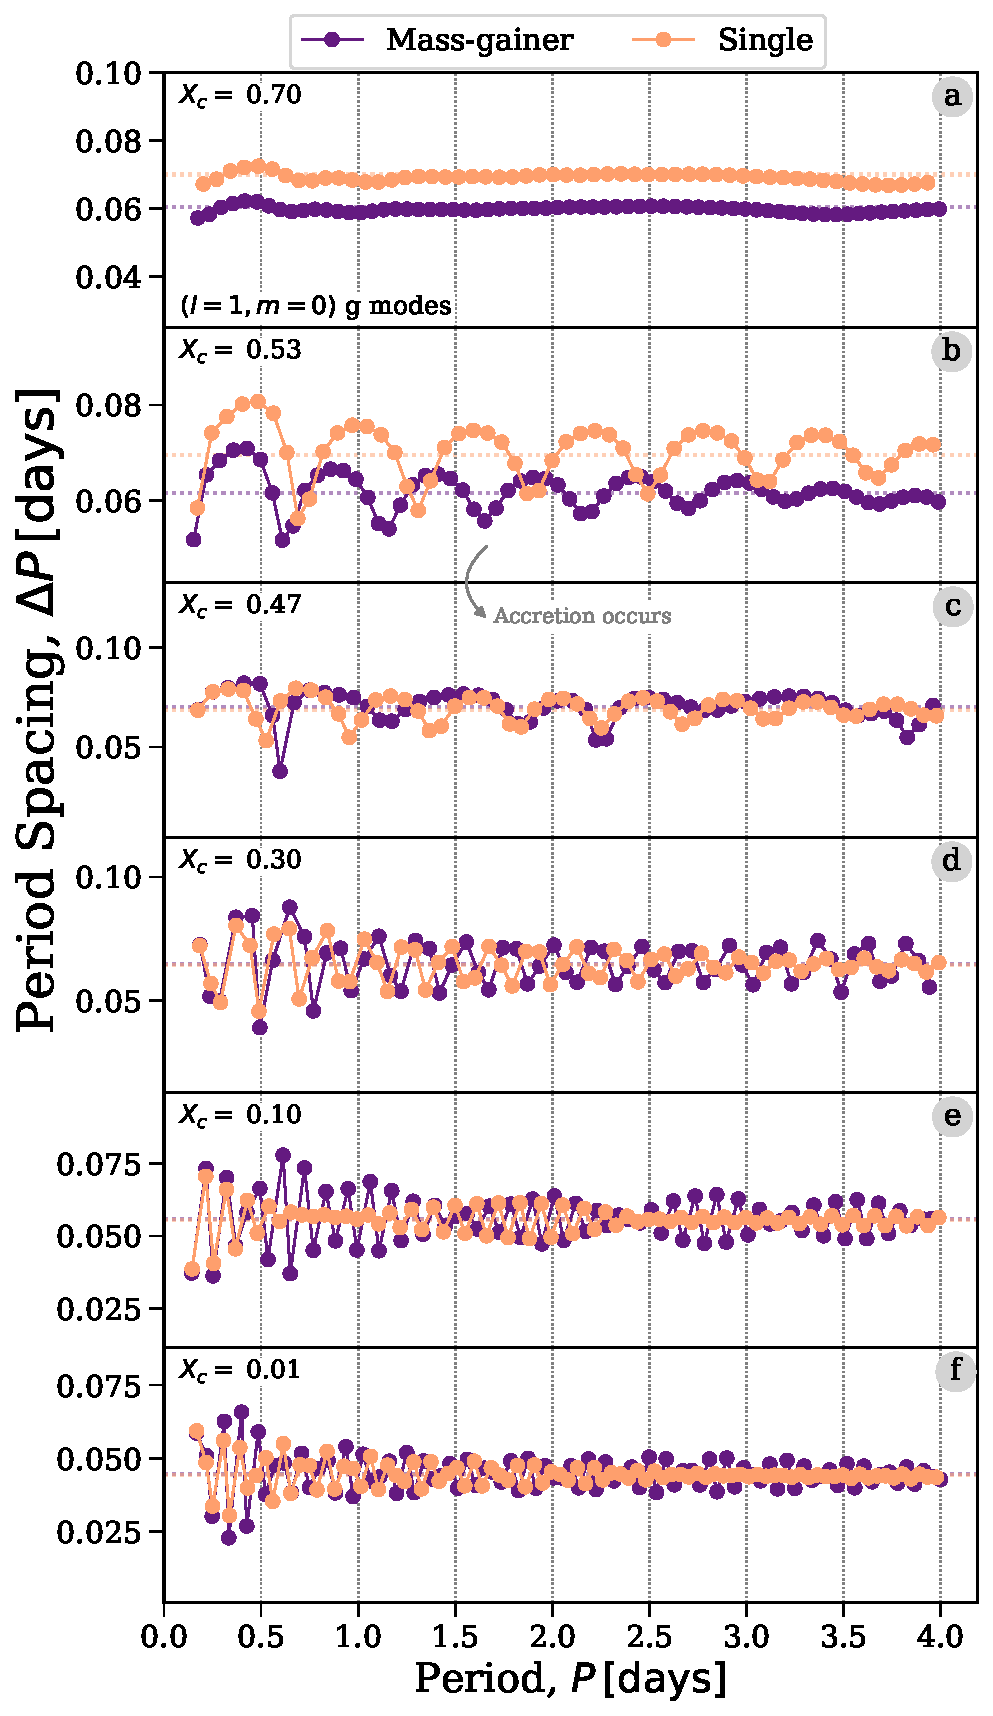
\includegraphics[width=\columnwidth]{figures/period_spacing_mdm20.pdf}
    \caption{As Figure~\ref{fig:XH_profiles}, but showing the period spacing patterns of the $\ell = 1, m = 0$ \gmodes. Asymptotic period spacings for each model are shown as dotted lines. We emphasise that the $y$-axis limits vary by panel.}
    \label{fig:period_spacing}
\end{figure}

In Figure~\ref{fig:period_spacing} we compare the period spacing pattern of a mass-gainer to that of an equivalent single star at different stages during their evolution. At the zero-age main sequence (in panel a), the period spacing pattern closely follows each star's asymptotic period spacing (denoted as dotted lines) due to the lack of any composition gradients. Early during the main sequence, immediately prior to mass transfer (in panel b), the pattern now displays some oscillation around the asymptotic value due to the chemical composition gradients that have developed outside of the core. Since this is currently pre-accretion, the stars have different masses and thus convective core sizes, resulting in an offset between their asymptotic period spacings.

In subsequent panels (c--f) there are several differences in the period spacing pattern, despite the fact that the stars now have the same mass and convective core size. The two main differences can be expressed in terms of amplitude and phase of oscillations in the period spacing pattern. Frequently in the stars' later evolution, we note that the amplitude of deviations from the asymptotic spacing are larger for the mass-gainer. This is because the mass-gainer contains regions with steeper chemical composition gradients, which more strongly impact the \bvf and thus the period of oscillations.

\help{It seems like the amplitude argument could be flawed, if this was true would we not only see amplitude differences in regions with phase differences?}

In addition, we find that the period spacing pattern shifts phase in certain regions for the mass gainer. This is most apparent in panel e, in which the patterns are out of phase for periods between ${\sim}1.5$--$3.2 \unit{days}$ and in-phase otherwise. These period-dependent shifts arise due to difference between the \bvf profiles occurring in the region of changing chemical composition. Modes that are sensitive to this region are shifted and so move out of phase, whilst other modes are insensitive to the differences from a single star and thus oscillate with the same periods.

\section{Discussion} \label{sec:discussion}
We have demonstrated that, compared to an equivalent single star, a mass-gainer shows significant differences in its period spacing pattern as a result of accretion altering its chemical composition gradient. In this Section we examine the implications of this result, considering both the impact on current inference modelling, as well as the potential for constraining mass transfer physics.

\subsection{Implications for inferring stellar properties}
Current work considers only single star evolution when inferring stellar properties from period spacing patterns. We have shown that these patterns are significantly changed as a result of mass transfer. Therefore, given that around $20\%$ SPB stars are expected to be in interacted binaries, current methodology may result in incorrect inferences.

We test how incorrect these inferences may be by fitting the period spacing pattern of our mass-gainer model assuming single star evolution. We use \texttt{GYRE} to compute the periods of $\ell = 1, m = 0$ \gmodes for our grid of single star models between 3 and 6\msun across the entire main sequence. We then perform a reduced $\chi^2$ fit for a given mass-gainer period spacing pattern with every single star model, at every timestep.

We match the periods of models independent of radial order, given that the exact radial order of an observed pulsation is not known a priori. In order to determine this matching we identify the offset, $\epsilon$, between the mass-gainer and single star radial orders that would result in the best fit for a chain of periods of consecutive radial order\footnote{We explored other techniques for determining this matching, such as using the longest chain of consecutive radial, and instead matching a single mode and using the next 20 modes. In each case we found very similar results.}. These chains are motivated by the fact that one would expect that, for a well fitting model, adjacent mass-gainer periods would match to adjacent single star periods.

We calculate the $\chi^2$ per degree of freedom for each model as
\begin{equation}
    \chi^2 = \frac{\sum_{i}^{N} (P_{{\rm mg}, i} - P_{{\rm s}, (i + \epsilon)})^2}{N - 1},
\end{equation}
where $P_{\rm mg}$ and $P_{\rm s}$ are the \gmode periods of the mass-gainer and single star models respectively, $N$ is the minimum of the number of periods in each model and $\epsilon$ is an offset in radial order between the models described above.

In Figure~\ref{fig:chi2_xc_0.2}, we show an example of this $\chi^2$ fitting. In this plot the mass-gainer model has a mass of $3.5 \msun$ and central hydrogen content of $X_c = 0.2$. However, the best fitting model when assuming single star evolution underestimates the mass at $3.1 \msun$ and significantly overestimates the central hydrogen content at $X_c = 0.4$, twice the true value. This best-fitting value is found along the degeneracy between mass and hydrogen content.

\begin{figure}[tb]
    \centering
    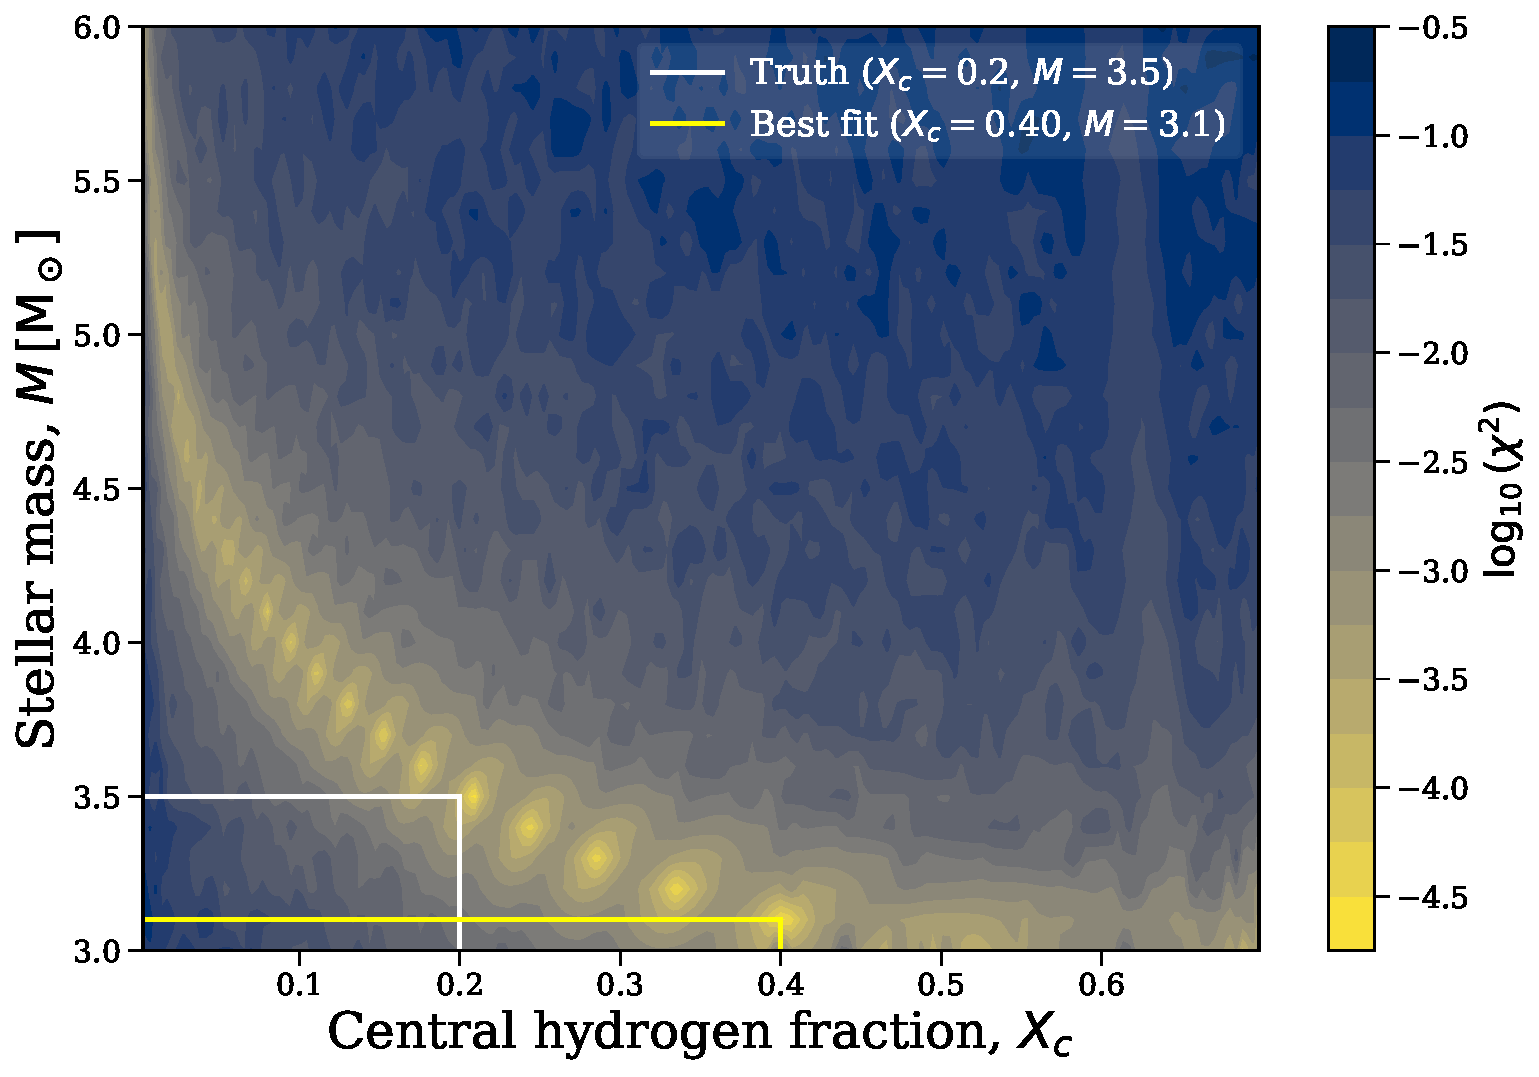
\includegraphics[width=\columnwidth]{figures/chi2_xc_0.2.pdf}
    \caption{Stellar properties can be inferred incorrectly when assuming single star evolution. $\chi^2$ values for fitting our mass-gainer model at $X_c$ with our entire grid of single star models. The true values and best fit are highlighted with lines.}
    \label{fig:chi2_xc_0.2}
\end{figure}

% \begin{table}[htb]
%     \centering
%     \begin{center}
%         \begin{tabular}{cc|cc}
%     \hline
%         \multicolumn{2}{c|}{Truth (Mass-gainer model)} & \multicolumn{2}{c}{Best fit (Single star model)} \\
%         Mass [\msun] & $X_c$ & Mass [\msun] & $X_c$\\ \hline
%         3.5 & 0.470 & 3.5 & 0.642\\
%         3.5 & 0.400 & 3.5 & 0.417\\
%         3.5 & 0.300 & 3.5 & 0.309\\
%         3.5 & 0.200 & 3.1 & 0.400\\
%         3.5 & 0.100 & 3.0 & 0.256\\
%         3.5 & 0.010 & 3.2 & 0.021\\ \hline
%     \end{tabular}
%     \end{center}
%     \caption{Comparison of best-fit single star models to mass-gainer model at different evolutionary stages.}
%     \label{tab:fits}
% \end{table}

We repeated this fitting procedure throughout the evolution of the mass-gainer model and summarise the results in Table~\ref{tab:fits}. Shortly after mass transfer ends (at $X_c = 0.47$), the best fit overestimates $X_c$ but accurately determines the stellar mass. As the star settles onto the main sequence, the best-fit improves, with mass and $X_c$ values very close to the true values. However, in the later stages of the star's main sequence evolution ($X_c \le 0.2$), the best-fit diverges from the true value again, significantly overestimating $X_c$ by at least a factor of 2 and consistently underestimating the stellar mass.

\begin{table}[htb]
    \centering
    \begin{tabular}{c|cc}
        \hline
        Mass-gainer & \multicolumn{2}{c}{Best fit (Single star model)} \\
        $X_c$ & $X_c$ & $M\, [\msun]$ \\ \hline
        0.47 & 0.642 & 3.5\\
        0.4 & 0.417 & 3.5\\
        0.3 & 0.309 & 3.5\\
        0.2 & 0.400 & 3.1\\
        0.1 & 0.256 & 3.0\\
        0.01 & 0.021 & 3.2\\ \hline
    \end{tabular}
    \caption{Comparison of best-fit single star models to mass-gainer model at different evolutionary stages. Columns show central hydrogen content, $X_c$, and stellar mass, $M$. In each case the mass-gainer model has a mass of $3.5 \msun$.}
    \label{tab:fits}
\end{table}

We therefore show that, though there are regimes within the main sequence in which using single star models may suffice for fitting mass-gainers, for a large fraction of the main sequence this will result in significant inaccuracies. The exact regimes in which these inaccuracies occur are likely mass and model dependent. Yet, given that the central hydrogen content of a star, as well how recently it may have undergone mass transfer, is generally unknown a priori, this implies one should be cautious when fitting a potential mass-gainer using single star models.

\subsection{Constraining mass transfer}

\begin{itemize}
    \item With independent measurements of parameters like age/composition you should be able to tell if period spacing pattern is off
    \item This can tell you about mass transfer
\end{itemize}

\todo{Write mass transfer constraint discussion}

\subsection{Caveats}\label{sec:caveats}
\paragraph{Rotation} Given this analysis acts as a proof of principle, we have limited the scope of our investigations by neglecting rotation in each model. Yet, in reality, we expect that SPB stars will rotate, and this will impact several aspects of our results. In particular, rotation may enhance mixing in the vicinity of the core and alter the chemical composition gradient, which is the key difference between the mass-gainer and single star models.

\paragraph{Diffusive mixing} We enforce a minimum diffusive mixing both as an attempt to counter the lack of rotational mixing and eliminate any numerical artifacts. Given diffusive mixing directly smooths the chemical composition gradient, the choice of the minimum value has also an impact on our results for the \bvf and period spacing pattern. However, as we demonstrate in Appendix~\ref{app:min_D_mix}, differences between the mass-gainer and single star models are still present for a wide-range of choices for this parameter.

\paragraph{Mass-gainer model} The mass-gainer model that we use is formed from a binary in which we artificially ended mass transfer once 0.5\msun of material was accreted. Although this choice is well motivated, since an accretor with rotation would quickly reach critical rotation and prevent further accretion, the choice may impact our results. Additionally, we only consider a single mass-gainer model for this proof of principle analysis and, though we expect the differences we find will be prevalent across a range of masses and periods, further work is necessary to confirm this.

\subsection{Future work}
\begin{itemize}
    \item Examine this for a grid of binary models
    \item Include rotation
    \item Apply \citet{Miglio+2008} framework to the distributions that we expect to see from mass transfer
\end{itemize}

\todo{Write future work subsection}

\section{Summary \& Conclusions} \label{sec:conclusion}

\todo{Write conclusions}

\begin{acknowledgements}
    We thank the Kavli Foundation and the Max Planck Institute for Astrophysics for supporting the 2023 Kavli Summer Program during which much of this work was completed. In particular, TW thanks Isabel Thapa, Stephen Justham and Selma de Mink for their incredible efforts in organising this program. TW also thanks Ruggero Valli for his help, and patience, with setting up \mesa on the MPA cluster and sharing the secret commands of \texttt{kinit} and \texttt{aklog}.
\end{acknowledgements}

\software{\mesa: The MESA EOS is a blend of the OPAL \citep{Rogers2002}, SCVH
\citep{Saumon1995}, FreeEOS \citep{Irwin2004}, HELM \citep{Timmes2000},
PC \citep{Potekhin2010}, and Skye \citep{Jermyn2021} EOSes. Radiative opacities are primarily from OPAL \citep{Iglesias1993, Iglesias1996}, with low-temperature data from \citet{Ferguson2005} and the high-temperature, Compton-scattering dominated regime by \citet{Poutanen2017}. Electron conduction opacities are from \citet{Cassisi2007} and \citet{Blouin2020}. Nuclear reaction rates are from JINA REACLIB \citep{Cyburt2010}, NACRE \citep{Angulo1999} and additional tabulated weak reaction rates \citet{Fuller1985, Oda1994, Langanke2000}.  Screening is included via the prescription of \citet{Chugunov2007}. Thermal neutrino loss rates are from \citet{Itoh1996}. Roche lobe radii in binary systems are computed using the fit of
\citet{Eggleton1983}.  Mass transfer rates in Roche lobe
overflowing binary systems are determined following the
prescription of \citet{Ritter1988}.\\ \texttt{GYRE} \citep{Townsend+2013, Townsend+2018}, \texttt{Astropy} \citep{astropy:2013, astropy:2018, astropy:2022}, \texttt{Python} \citep{python}, \texttt{numpy} \citep{numpy}, \texttt{pandas} \citep{pandas_1.4.2, pandas_paper}, \texttt{matplotlib} \citep{matplotlib}, \texttt{scipy} \citep{Virtanen+2020}}

\bibliographystyle{aasjournal}
\bibliography{bibs/paper, bibs/mesa, bibs/software}{}

\restartappendixnumbering

\allowdisplaybreaks
\appendix

\section{Importance of choice of minimum diffusive mixing}\label{app:min_D_mix}

In our \mesa models we set a minimum diffusive mixing coefficient, $D_{\rm min}$, in order to account for mixing processes not included in our model and to mix over unphysical numerical composition gradients. For our models analysed in this paper we set $D_{\rm min} = 20 \unit{cm^2}{s^{-1}}$, in this Appendix we explore the impact that this choice has on our results.

\begin{figure}[b]
    \centering
    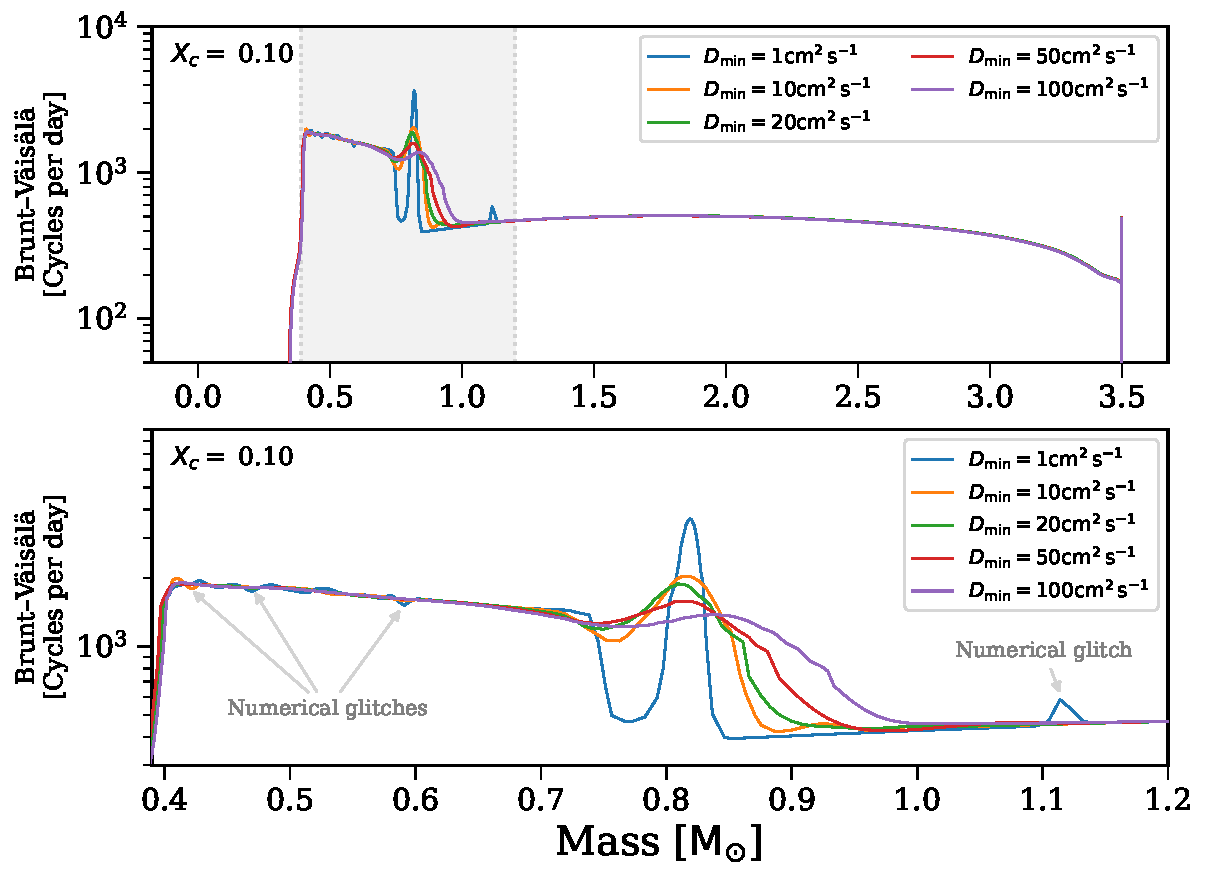
\includegraphics[width=\columnwidth]{figures/min_D_mix_comparison.pdf}
    \caption{Comparison of the impact of changing the \mesa miniumum diffusive mixing parameter, $D_{\rm min}$, on the \bvf profile. Bottom panel zooms in on the highlighted range in the top panel. Annotations highlight numerical glitches in low $D_{\rm min}$ models.}
    \label{fig:min_D_mix}
\end{figure}

We repeated our binary \mesa simulations for four additional choices of $D_{\rm min}$, ranging from $1 - 100 \unit{cm^2}{s^{-1}}$. In Figure~\ref{fig:min_D_mix} we compare the \bvf profiles of these models at a central hydrogen abundance of $X_c = 0.1$, where the lower panel zooms in on the highlighted region in the upper panel. There are significant differences in the profiles between the different models. As one may expect, lower mixing coefficients lead to steeper composition gradients and therefore sharper features in the \bvf and stronger signals in the period spacing pattern.

However, an overly low choice of $D_{\rm min}$ leads to numerical glitches in the composition gradient and the \bvf profile. We highlight this in Figure~\ref{fig:min_D_mix}, where glitches are clearly visible in both the $D_{\rm min} = 1 \unit{cm^2}{s^{-1}}$ and $D_{\rm min} = 10 \unit{cm^2}{s^{-1}}$ models.

We explored a more dense grid of $D_{\rm min}$ models and found that $D_{\rm min} = 20 \unit{cm^2}{s^{-1}}$ was the smallest level of mixing that still removed numerical glitches, which informed our selection of this model as the default choice in this paper. This level of mixing is not unexpected, since mass transfer will likely induce rotation in the accretor \citep{Packet+1981} and this leads to rotational mixing.

\begin{figure}[hbt]
    \centering
    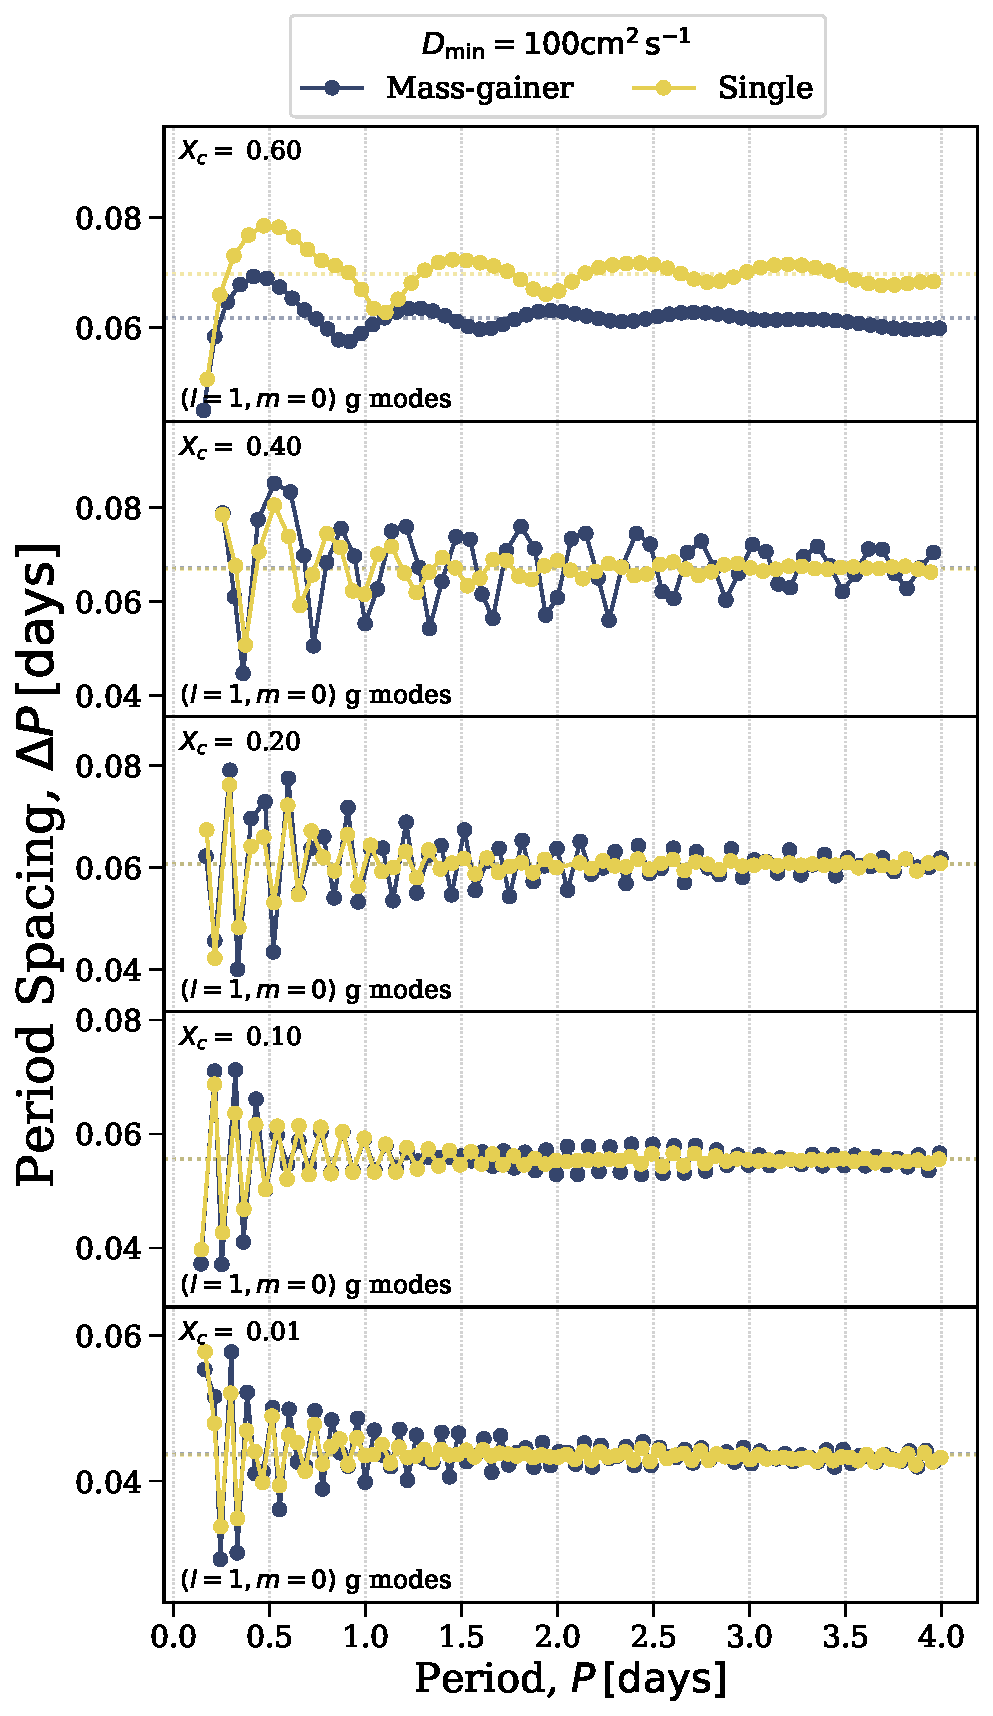
\includegraphics[width=0.9\columnwidth]{figures/period_spacing_mdm100.pdf}
    \caption{As Figure~\ref{fig:period_spacing}, but with the minimum diffusive mixing coefficient set to $D_{\rm min} = 20 \unit{cm^{2}}{s^{-1}}$.}
    \label{fig:period_spacing_mdm100}
\end{figure}

We stress that the qualitative differences between the mass-gainer and single star in the period spacing patterns remain the same for all choices of $D_{\rm min}$ that we explored. To highlight this point we show the period spacing pattern for the model with $D_{\rm min} = 100 \unit{cm^{2}}{s^{-1}}$ in Figure~\ref{fig:period_spacing_mdm100}. Despite slight differences to the exact shape of the pattern, we still find the same features of (i) stronger $\Delta P$ for mass-gainers and (ii) regions in which the period spacing is in-phase and regions in which it is out of phase between the mass-gainer and single star.

\section{\mesa Resolution Tests}\label{app:res_tests}
\texttt{delta\_mesh\_coeff} time
\tom{Check results hold with higher res}

\end{document}